\subsection{Spatial clusters}
\label{subsec:results-lisa}

The regression treats cells as independent, which they are not. The bivariate Moran statistic provides the global test, and it rejects that independence in every scenario. In Curitiba $I = 0.373$ under \texttt{thermal}, and in Porto Alegre $0.362$ under \texttt{flood} and $0.410$ under \texttt{flood+landslide}, all at $p = 0.001$. Adding vegetation lowers the global statistic in Curitiba to $0.258$ under \texttt{thermal+green}$, and adding landsliding lowers it in Porto Alegre to $0.165$ under \texttt{landslide}$, which is what the drop in explained variance already indicated.

The local indicators locate where that association sits. They separate the cells whose value of the SDI and whose time increase are both high (High-High) or both low (Low-Low) from the two discordant classes, high deprivation with low increase (High-Low) and low deprivation with high increase (Low-High). Cells not significant at $p \le 0.05$ receive no class. Table~\ref{tab:results-lisa} gives the share of the grid in each class.

\begin{table}[htbp]
\centering
\caption{Share of cells in each local bivariate cluster between the SDI and the per-cell increase in access time, as percentage of the grid. Global Moran $I$ and the share of significant cells are given for each scenario.}
\label{tab:results-lisa}
\fontsize{9}{9.6}\selectfont
\setlength{\tabcolsep}{4pt}
\begin{tabular}{llrrrrrr}
\hline
City & Scenario & Moran $I$ & Sig.\ (\%) & High-High & Low-Low & High-Low & Low-High \\
\hline
Curitiba & \texttt{thermal} & 0.373 & 37.3 & 7.6 & 20.5 & 5.8 & 3.3 \\
Curitiba & \texttt{thermal+green} & 0.258 & 35.1 & 8.4 & 16.5 & 6.4 & 3.8 \\
Curitiba & \texttt{thermal+demo} & 0.373 & 36.5 & 7.3 & 20.1 & 5.8 & 3.3 \\
Curitiba & \texttt{thermal+green+demo} & 0.369 & 37.0 & 8.2 & 19.9 & 5.6 & 3.3 \\
Porto Alegre & \texttt{flood} & 0.362 & 50.6 & 11.4 & 19.6 & 18.9 & 0.7 \\
Porto Alegre & \texttt{landslide} & 0.165 & 51.7 & 2.9 & 11.6 & 36.6 & 0.6 \\
Porto Alegre & \texttt{flood+landslide} & 0.410 & 43.7 & 8.8 & 22.3 & 12.3 & 0.3 \\
\hline
\end{tabular}
\end{table}

\begin{figure}[htbp]
\centering
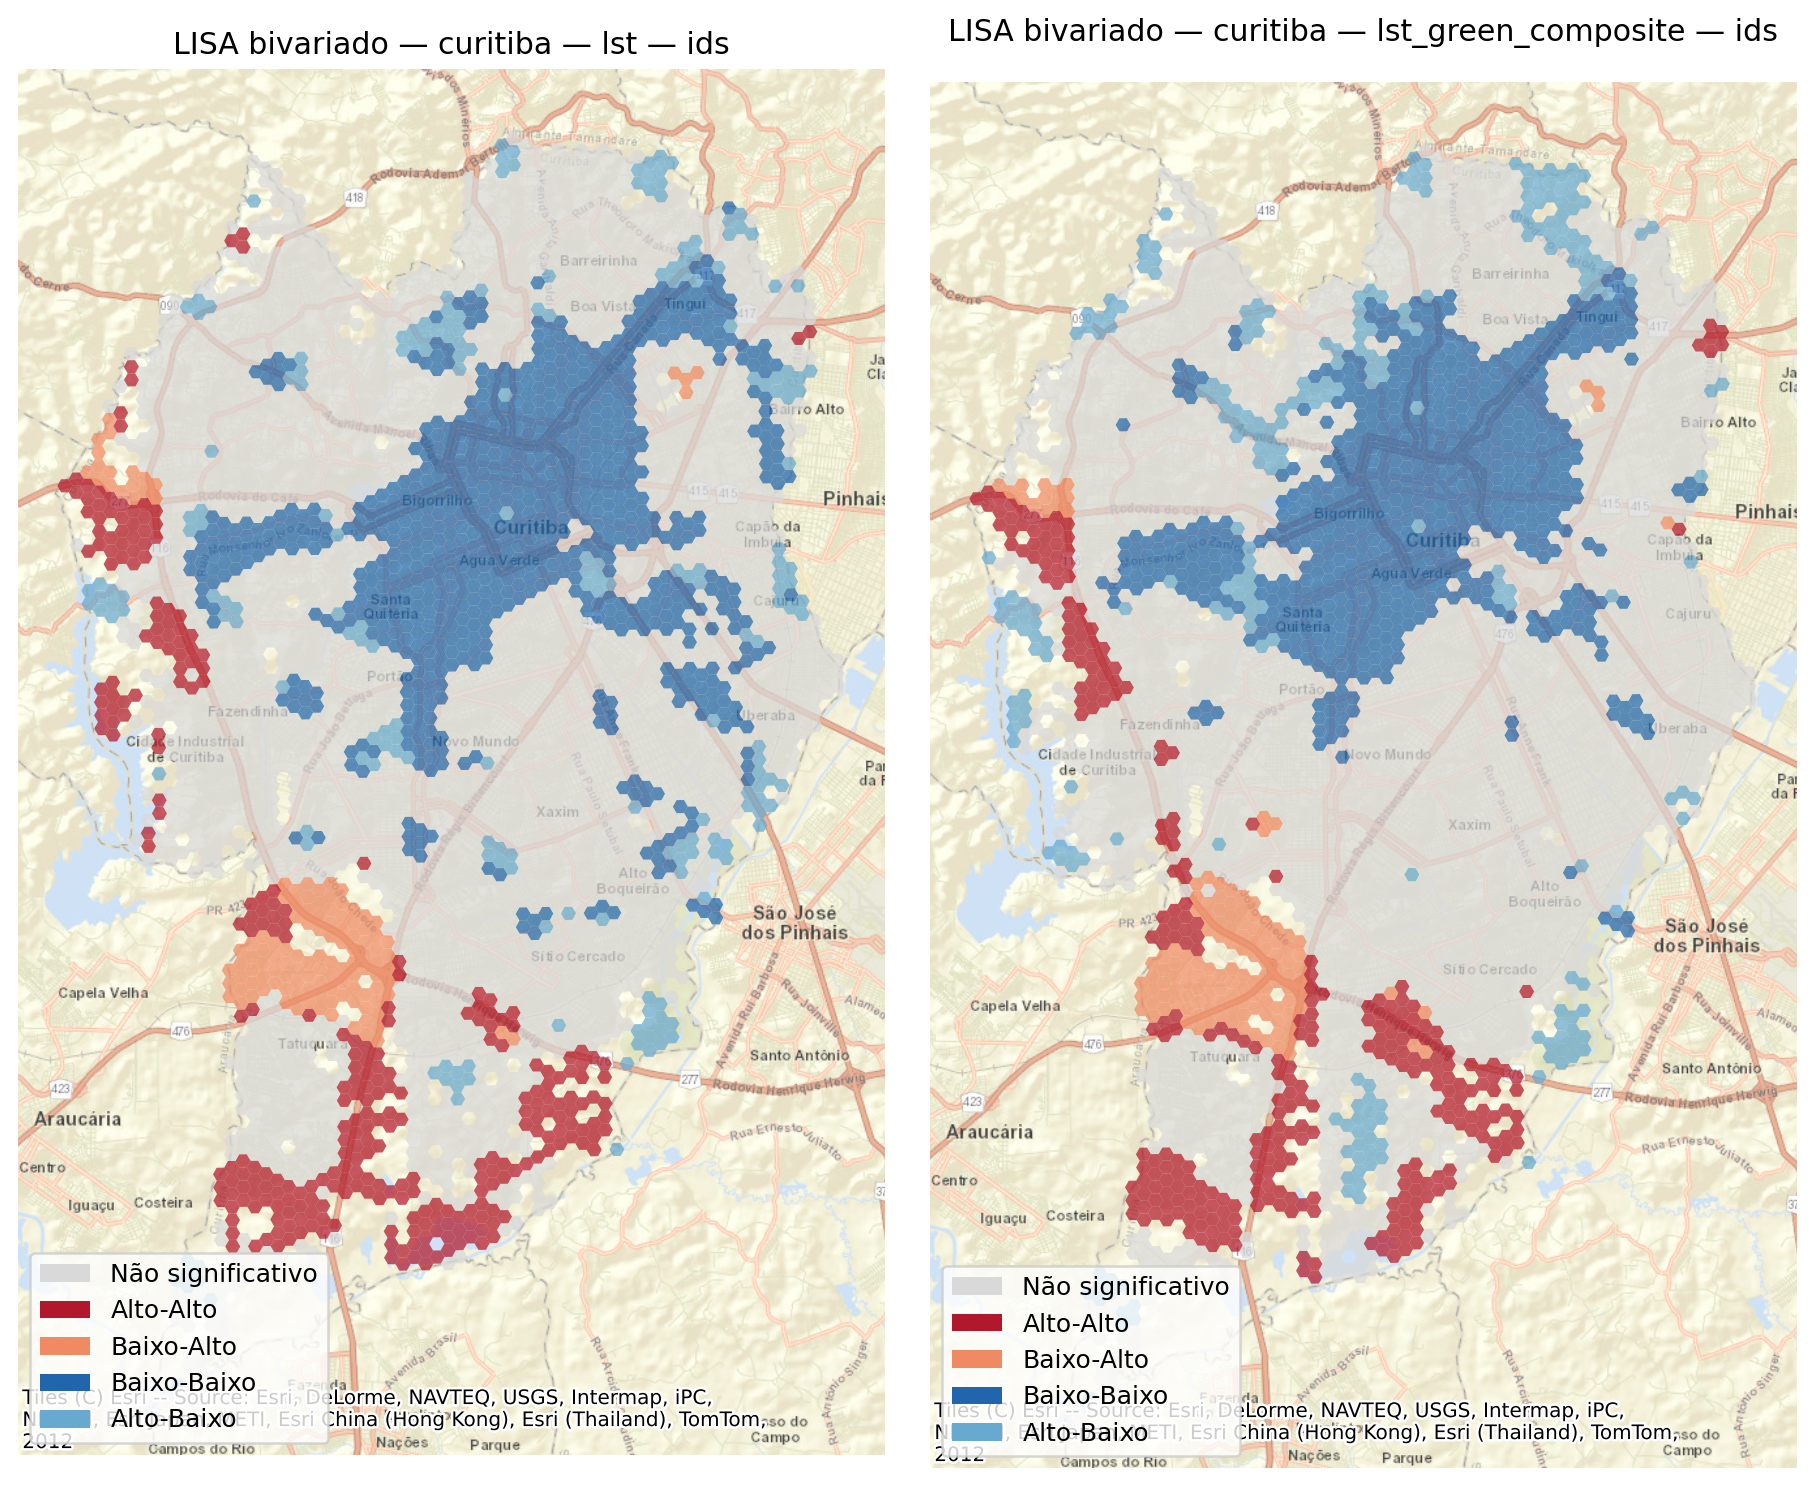
\includegraphics[height=0.30\textheight]{figs/lisa_curitiba.png}
\caption{Local bivariate clusters between the SDI and the per-cell increase in access time, Curitiba, under \texttt{thermal} (left) and \texttt{thermal+green} (right). Grey cells are not significant at $p \le 0.05$.}
\label{fig:results-lisa-curitiba}
\end{figure}

In Curitiba (Figure~\ref{fig:results-lisa-curitiba}), the Low-Low class accounts for 16.5\% of the grid under \texttt{thermal+green} against 8.4\% in High-High. That asymmetry reproduces the aggregate result. The large continuous core of the city has both low deprivation and no time increase, while the High-High clusters form separate patches at the western edge and along the southern corridor, where the two conditions coincide. The clusters that remain under \texttt{thermal+green} overlap the tracts the tree cover does not reach, which is the income axis doing the work the regression attributed to it. The vegetation also thins the Low-Low core from 20.5\% under \texttt{thermal} to 16.5\%, as the shade removes part of the delay from the centre and some central cells fall back under the significance threshold.

\begin{figure}[htbp]
\centering
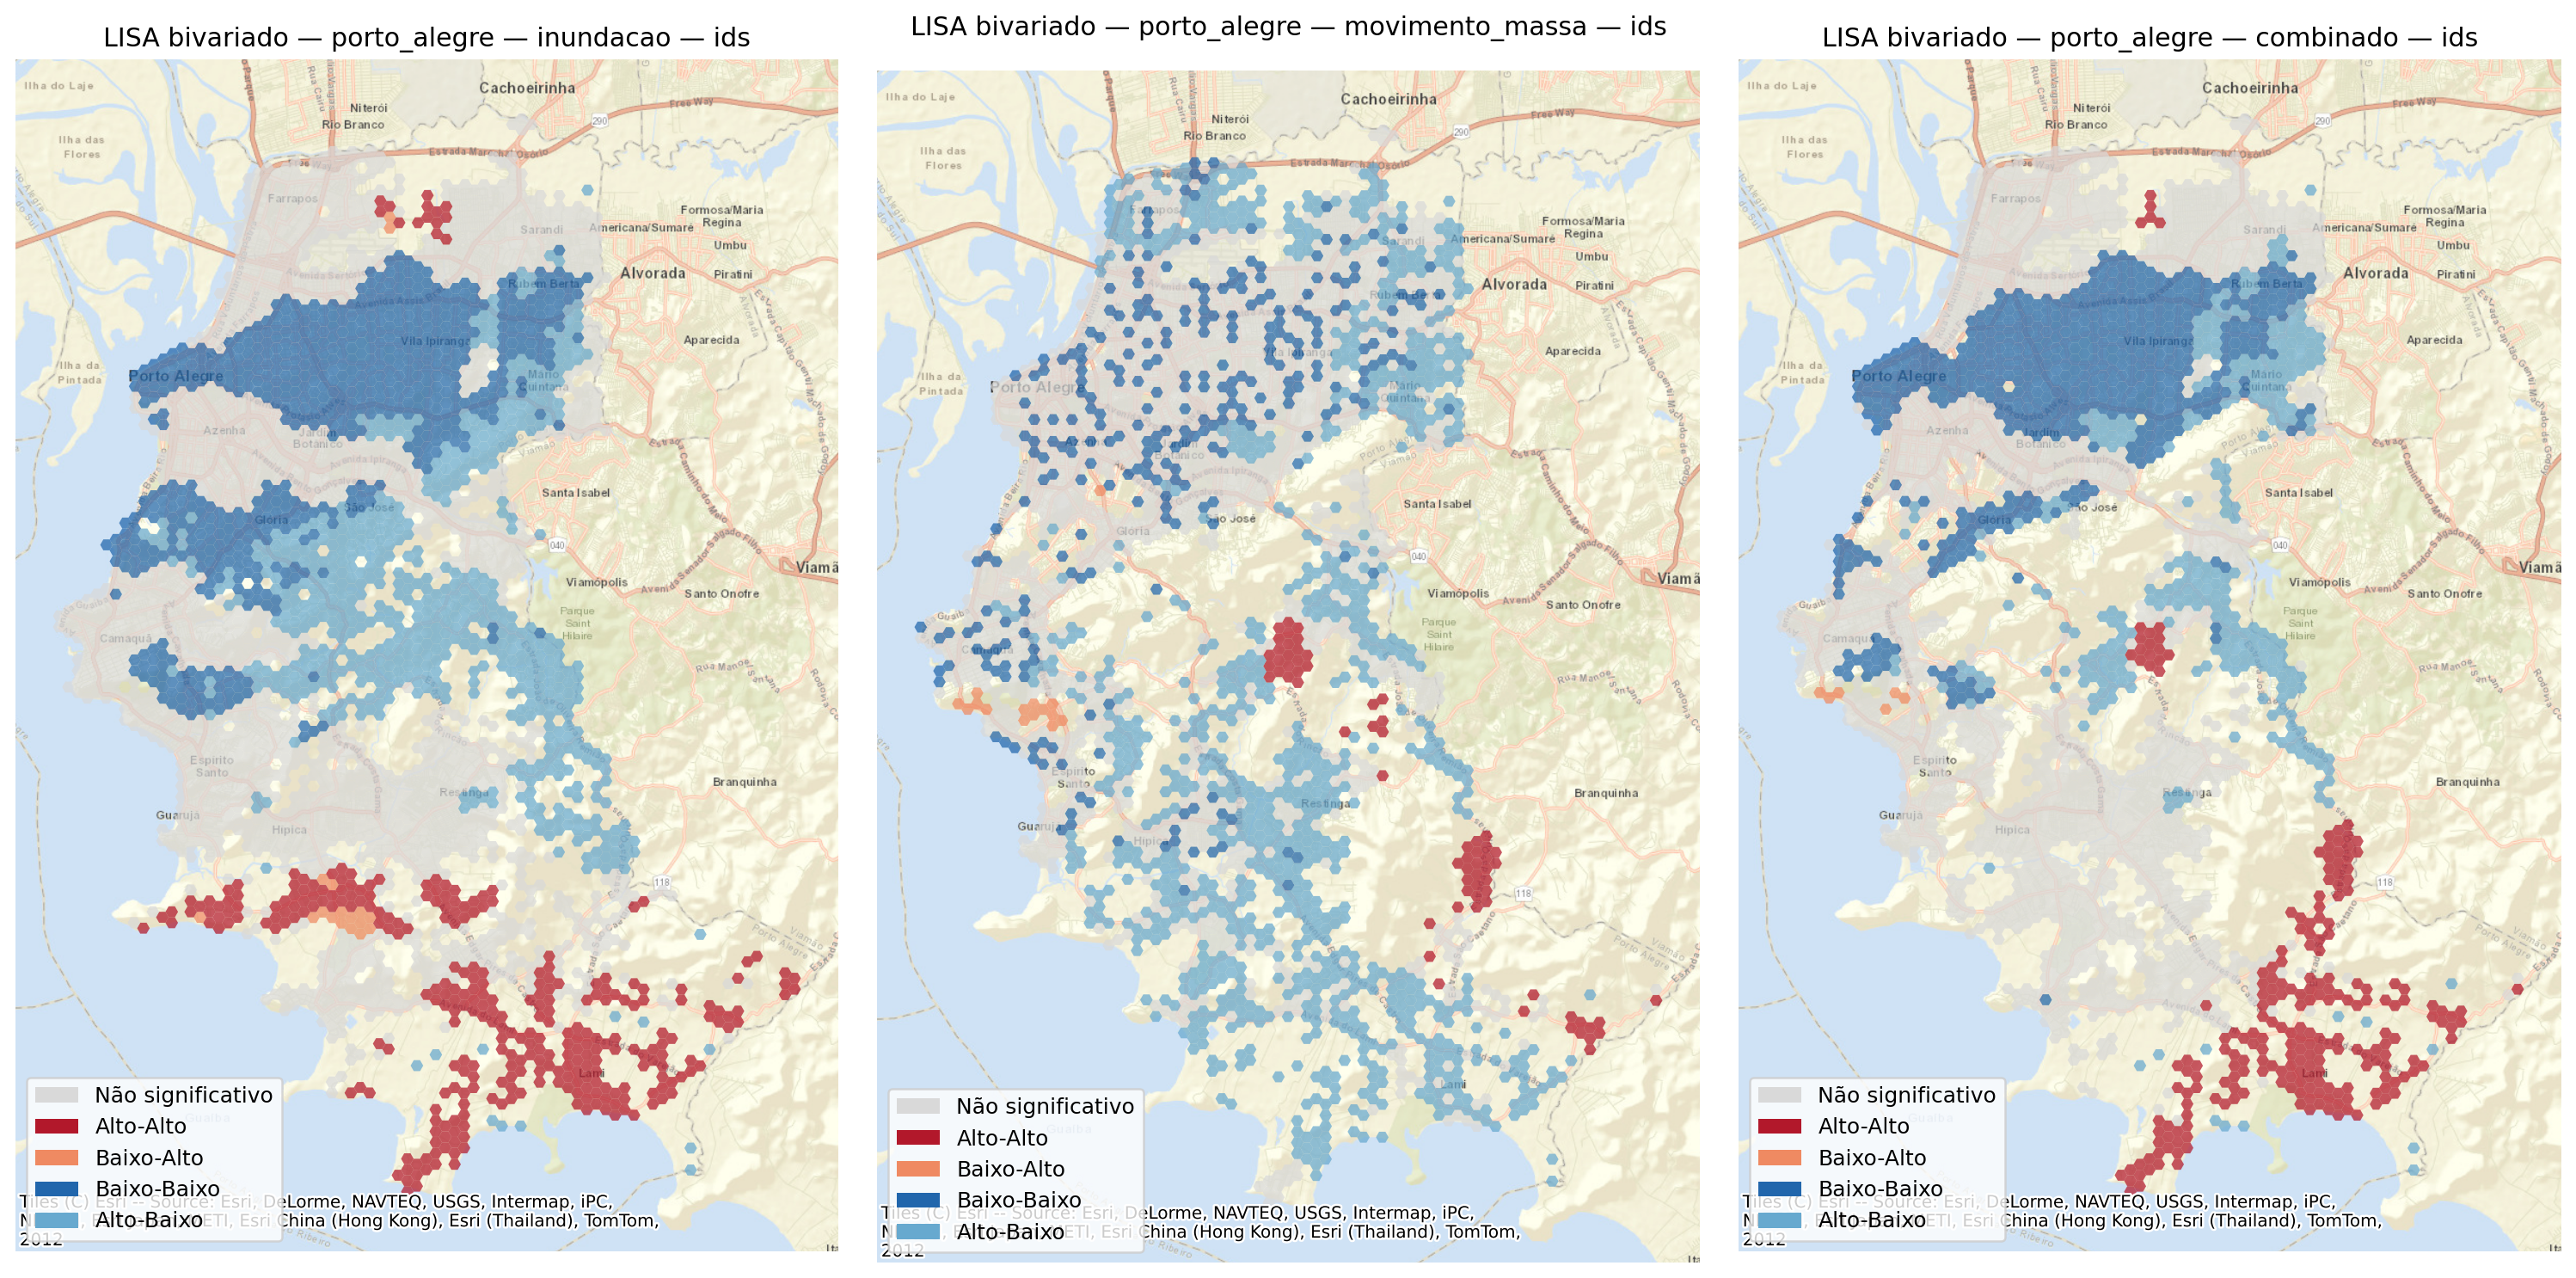
\includegraphics[height=0.26\textheight]{figs/lisa_porto_alegre.png}
\caption{Local bivariate clusters between the SDI and the per-cell increase in access time, Porto Alegre, under \texttt{flood} (left), \texttt{landslide} (centre) and \texttt{flood+landslide} (right). Grey cells are not significant at $p \le 0.05$.}
\label{fig:results-lisa-porto-alegre}
\end{figure}

Porto Alegre produces a signature the global statistic alone would hide (Figure~\ref{fig:results-lisa-porto-alegre}). Under \texttt{flood}, High-Low reaches 18.9\% of the cells, as large as the 19.6\% of Low-Low. Cells inside the floodplain lose time because the inundation reaches them by the polygon. Under \texttt{landslide} the same class grows to 36.6\%, and High-High falls to 2.9\%. The slope polygons intersect the city where deprivation is low, so \texttt{landslide} in this municipality concentrates loss of access in the better-served areas. Under \texttt{flood+landslide} the classes rebalance, High-High at 8.8\% and Low-Low at 22.3\%, and the High-High clusters become contiguous along the southern periphery, which is the pattern of a compound exposure acting on a network whose service provision already follows the same gradient.

Taken together, the results show the mechanism responding to the three properties the scenarios were built to exercise. It distinguishes continuous from discrete evidence, it distinguishes a delay from an interruption, and it composes layers without collapsing them into an average. Whether the magnitudes correspond to what would be observed in an actual event is a question the scenarios do not answer, and the next section takes it up.
